\chapter{A Coordinated Team of Autonomous Robots for the Rapid Assessment of
  Water Quality}\label{ch:robot-team}

As outlined in Chapter~\ref{ch:intro}, the accurate assessment of water
quality is essential for monitoring ecosystem health and ensuring the safety of
water resources. A plethora of physical parameters
influence local water quality such as turbidity, dissolved organic matter, chlorophyll
concentrations, and suspended particulate matter. Importantly, many of these
contribute measurably to the optical properties of water bodies via
their impact on the scattering and absorption of incident light. Hyperspectral
imaging, which enables the measurement of radiometric quantities
across hundreds of individual wavelength bins, offers a powerful tool for
assessing these parameters. By detecting the subtle variations in
reflectance across ultraviolet (UV), visible, and Infrared (IR) wavelengths,
hyperspectral imaging enables the differentiation of various water constituents
in complex environments.

In this chapter, we first introduce relevant concepts from radiometry and their
relationship to the measurements made by hyperspectral imagers. We then
describe a variety of physical parameters relevant for the assessment of water
quality and their manifestations in radiometric data. Armed with this
information, we then present a robotic team incorporating both
drone-based hyperspectral imaging and autonomous in situ data collection with an
autonomous boat. Carefully orchestrating the collection of hyperspectral
images (HSI) coincident with reference data for water quality parameters of
interest allows us to collect data volumes in a few minutes comparable to
decades-long satellite campaigns.

The sensing framework described in this chapter has been published in
\cite{robot-team-1} and was utilized for the studies presented in
Chapters~\ref{ch:robot-team-supervised}, \ref{ch:robot-team-gtm}, and \ref{ch:robot-team-gsm}.


\section{Light and Water}\label{sec:imaging}

Perhaps the greatest achievement of 19th century physics was the unification of
electricity and magnetism by James Clerk Maxwell in which the phenomenon of
light propagation is fundamentally described by oscillations in the electric and
magnetic fields. Therefore, let us first consider a motivating example of
electromagnetic plane waves propagating in a dielectric medium before relating them to
the radiometric measurements made by physical sensors. Recall that Maxwell's
equations in matter are given by
\begin{equation}\label{eq:maxwell}
  \begin{aligned}
    \nabla \cdot \mathbf{D} &= \rho_f, & \nabla \times \mathbf{E} &= - \partial_t \mathbf{B}, \\
    \nabla \cdot \mathbf{B} &= 0, & \nabla \times \mathbf{H} &= \mathbf{J}_f + \partial_t\mathbf{D},
  \end{aligned}
\end{equation}
where $\rho_f$ is the free charge density and $\mathbf{J}_f$ is the free current
density. For linear media of permittivity $\epsilon$, and permeability $\mu$, we
have $\mathbf{D}=\epsilon\mathbf{E}$ and $\mathbf{H}=\frac{1}{\mu}\mathbf{B}$.
In a region where $\rho_f=0$ and $\mathbf{J}_f=0$, these equations reduce to the
wave equation for $\mathbf{E}$ and $\mathbf{B}$, admitting traveling plane-wave
solutions.

A monochromatic plane-wave traveling in the $\hat{x}$ direction is given by
\begin{equation}\label{eq:travelling-wave}
  \begin{aligned}
    \mathbf{E} &= \bar{E}_0\exp(i(\kappa x - \omega t))\hat{y}, \\
    \mathbf{B} &= \bar{B}_0\exp(i(\kappa x - \omega t))\hat{z},
  \end{aligned}
\end{equation}
where $\bar{E}_0$ and $\bar{B}_0$ are complex numbers
(absorbing the phase). Equation~\ref{eq:travelling-wave} trivially satisfies
$\nabla \cdot \mathbf{D} = 0$ and $\nabla \cdot \mathbf{B} = 0$. Substitution into
the remaining equations yields the familiar dispersion relation for
electromagnetic waves:
\begin{equation}
  \kappa^2 = \omega^2\mu\epsilon
\end{equation}
with a wave velocity $v=1/\sqrt{\mu\epsilon}$.

Allowing for $\sqrt{\mu\epsilon}$ to be complex, we can decompose $\kappa$ into
\begin{equation}
  \kappa = \frac{2\pi m}{\lambda}
\end{equation}
where $m=n - ik$ is the \textit{complex index of refraction}. Substituting this expression
into Equation~\ref{eq:travelling-wave} and taking the real part, we obtain
\begin{equation}\label{eq:wave-real}
  \begin{aligned}
    \mathbf{E} &= E_0\exp\left(-\frac{2\pi k x}{\lambda}\right)\cos\left(  \frac{2\pi n x}{\lambda} - \omega t  + \phi \right) \hat{y} \\
    \mathbf{B} &= B_0\exp\left(-\frac{2\pi k x}{\lambda}\right)\cos\left(  \frac{2\pi n x}{\lambda} - \omega t  + \phi \right) \hat{z} \\
  \end{aligned}
\end{equation}

Instruments like hyperspectral imagers do not measure
the time-dependent amplitudes of the electric and magnetic fields. Instead, they
detect energy carried by these fields into a surface. This energy
flow is characterized by the Poynting vector, $\mathbf{S} =
\frac{1}{\mu}\mathbf{E}\times\mathbf{B}$ which has units of $W/m^2$, in other
words, the energy flux through a surface. Additionally, the sample rates of realistic
instruments are much longer than oscillations in $\mathbf{E}$ and $\mathbf{B}$ so
that the time-averaged Poynting vector $\langle
\mathbf{S} \rangle$ is what is really measured. Given that $\langle  \cos^2(\theta) \rangle =
1/2$, this results in
\begin{equation}
  \langle \mathbf{S} \rangle = \frac{1}{2}\sqrt{\frac{\epsilon}{\mu}}E_0^2\exp\left(-\frac{4\pi k x}{\lambda}\right) \hat{x}.
\end{equation}

Here we see an important consequence of considering a complex index of reaction:
the quantity $a(\lambda)=4\pi k/\lambda$ is called the \textit{absorption coefficient}
which characterizes the amount of incident radiation absorbed by the medium as a
function of the penetration distance $x$. In low-turbidity coral reefs this helps
explains why red colors become muted at increasing depths. Finally, we note that
for a homogeneous solution containing $n$ chemicals, the Bouguer-Beer-Lambert law
relates the total absorption coefficient to each chemical concentration via
\begin{equation}
  a(\lambda) = \sum_i^n c_i\varepsilon_i(\lambda)
\end{equation}
where $c_i$ is the concentration of the $i$-th chemical species in the solution,
and $\varepsilon_i(\lambda)$ is the wavelength-dependent molar absorption
coefficient. The connection between the concentration of constituents in the
water to the interaction of a mixture with incident light motivates the
assessment of water quality by spectroscopic techniques.

\subsection{Radiometry}

\textit{Radiometry} is the science of the measurement of electromagnetic energy
and involves a number of derived quantities. As outlined in the previous
section, most optical and spectroscopic instruments do not directly measure the
oscillations in the electric and magnetic fields, but rather the energy they
transport into a sensing element. 

The \textit{spectral radiance} is defined as
\begin{equation}
  L(\mathbf{x}, t, \hat{\xi}, \lambda) = \frac{\partial^4 Q}{\partial t \partial A \partial \Omega \partial \lambda},
\end{equation}
or in words, the amount of incident radiant energy per area per
second, per solid angle, per wavelength. Importantly, the spectral radiance
depends on the sampling position $\mathbf{x}$ and time $t$ as well as the wavelength
$\lambda$ and direction of light $\hat{\xi}$. Historically many different
conventions for naming radiometric quantities have been used. We follow the
conventions used in \cite{mobley-text} for which the prefix \textit{spectral} is
used to indicate the explicit \textit{per-wavelength} dependence of a
radiometric quantity. $L$ is the fundamental measured quantity which captures
the spatial, temporal, spectral, and orientation dependencies of the light field.

When an instrument samples light from \textit{all} possible directions passing
through a collection area, then the
measured quantity is the \textit{spectral irradiance}. Naturally, this quantitiy
depends on the orientation of the sensor. For example, the \textit{downwelling
  spectral irradiance}, $E_d$ is defined by
\begin{equation}
  E_d(\mathbf{x}, t, \lambda) = \int_0^{2\pi} \int_0^{\pi/2}L(\mathbf{x}, t, \theta, \phi, \lambda)\cos\theta \sin\theta d\theta d\phi
\end{equation}
where the factor of $\cos\theta$ accounts for the apparent area at an angle
$\theta$ from the surface normal.

Different materials lead to different distributions of scattered light. For
\textit{specular} materials such as polished mirrors or the air-water interface, light
reflected at the surface leaves at an angle identical to the angle of incidence.
The polar opposite of a specular material is a \textit{Lambertian}, or perfectly
diffuse material. Light scattering off of a Lambertian surface is distributed
equally in all directions so that $L$ is independent of $\theta$ and $\phi$. As
a consequence, the spectral irradiance of light from a Lambertian surface is
\begin{equation}
  E = \int_0^{2\pi}\int_0^{\pi/2} L(\mathbf{x}, \lambda)\cos\theta \sin\theta d\theta d\phi = \pi L
\end{equation}

Given measurements for the downwelling (incident) and upwelling spectral
irradiances, the \textit{reflectance} is defined by their ratio:
\begin{equation}
  \rho(\mathbf{x},\lambda) = \dfrac{E_u(\mathbf{x}, \lambda)}{E_d(\mathbf{x}, \lambda)}.
\end{equation}
This quantity is valuable as it extracts the useful signal from an image by
\textit{dividing out} the spectrum from the lighting source, in this case,
incident solar radiation. Hyperspectral imagers typically measure spectral
radiance but can be calibrated to obtain the reflectance.

\subsection{Optical Properties of Water Bodies}\label{sec:optical-properties-water}

The formulation of Maxwell's equations in Equation~\ref{eq:maxwell} treats
macroscopic media as continuous. However, at atomic scales, bodies of water
consist of collections of molecules (\ce{H2O} and other dissolved substances)
together with particulates which vary in size. The interaction of light with
these particles can be approximated by the interaction of light with dielectric
spheres with a specific radius and (potentially complex) index of refraction.
The general solution for the scattered intensity field of light by a dielectric
sphere of \textit{any} radius is known as \textit{Mie Theory} and involves
highly complicated expressions of infinite series of spherical multi-pole
expansions which can be evaluated numerically.

A special case for elastic scattering by particles with a diameter $d <<
\lambda$ is known as \textit{Rayleigh Scattering}. In this regime, the scattered
intensity obeys
\begin{equation}
  I = I_0  \left( \frac{2\pi}{\lambda} \right)^4 \left( \frac{d}{2} \right)^6 \left( \frac{1 + \cos^2\theta}{2R^2} \right)
\end{equation}
where $\theta$ is the scattering angle, $R$ is the distance from the particle to
the measurement point, and $n$ is the (real) index of refraction. Lord Rayleigh
used the $\lambda^{-4}$ dependence of this expression to explain why the sky is
blue: atmospheric particles (which we now understand to be gas molecules) with
diameters much smaller than visible wavelengths scatter blue light
much more than red light.

In addition to scattering, molecules and particulates can absorb incident light
according to their specific structure. For pure water, electronic transitions
lead to absorption in the UV while rotational and vibrational modes are relevant
at longer wavelengths. Critically, there is a transparent \textit{window} of low
absorption for visible wavelengths which enables aquatic life to access solar
energy.

Water bodies contain a variety of constituents leading to a continuous size
distribution from chemicals at the atomic scale ($\sim$$0.1$ nm) up to aquatic
animals ($\sim$$1$ m). These components are traditionally
classified into dissolved or particulate matter of organic or inorganic origin.
Most water bodies contain a variety of dissolved salts. For ocean waters these
account for roughly 3.5\% by weight while fresh water bodies tend to contain
trace amounts. Natural waters also contain a variety of dissolved organic
compounds produced by the decay of plant matter. These compounds mostly include
fulvic and humic acids which impart a yellowish-brown color in sufficient
concentrations and are referred to in the literature as \textit{colored
  dissolved organic matter} (CDOM) \cite{cdom-acids}. Inorganic particulate
matter in natural waters is largely due to the weathering and erosion of rocks
and soils while organic particulates include bacteria, phytoplankton,
zooplankton, and larger organic detritus.

Light absorption by CDOM can be reasonably modeled using an exponential function
of the form
\begin{equation}
  a(\lambda) = a(\lambda_0)\exp(-S_g(\lambda - \lambda_0))
\end{equation}
for a reference wavelength $\lambda_0$ \cite{aurin2018remote}. The exact
value of the spectral slope $S_g$ depends on the proprotions of specific types
of CDOM with typical values on the order of $\sim$$0.01$.

Absorption by phytoplankton and many other organic sources is largely due to
photosynthetic pigments with cells such as chlorophyll. Chlorophyll a
absorption is strongest for blue and red wavelengths with peaks at
$\lambda\approx 430$ nm and $\lambda\approx 665$ nm, respectively. Other
relevant pigments include phycoerythrin and phycocyanin  which occur in
blue-green algae. Estimations of their concentration from remote sensing imagery
has been used to track the evolution of harmful algal blooms which often occur
due to increased nutrient concentrations from agricultural and urban runoff
\cite{algal-blooms-rs}.

Lastly, we note that in addition to scattering and absorption, many chemicals
such as crude oil and organic components such as CDOM and chlorophyll undergo
fluorescence when excited at appropriate wavelengths. For example, CDOM excited
by UV light with $\lambda\in[250, 400]$ nm will emit at wavelengths in
$\lambda\in[400, 500]$ depending on the specific types of organic compounds
\cite{cdom-fluorescence}. Fluorometers calibrated for these excitation
and emission properties can therefore be used for in situ assessment of many
water constituent concentrations.

\section{Coordinated Robot Teams}

For decades, multi-spectral imagers which sample a small number of
broad wavelength bands have seen widespread use in
the remote sensing community as a means to take advantage of the wealth of
information contained in the reflectance spectra of materials. Multi-spectral imagers,
like those deployed on MODIS, Sentinel 2, and other satellite platforms, include
wavelength bands ranging from the near-UV,
through the visible spectrum, and into the Infrared and have been applied in a
variety of domains from tracking land change, characterizing deforestation,
monitoring erosion, evaluating crop health, and many others
\cite{remote-sensing-foliage, remote-sensing-applications, thenkabail-indices}.

\begin{figure}[!hbt]
  \centering
  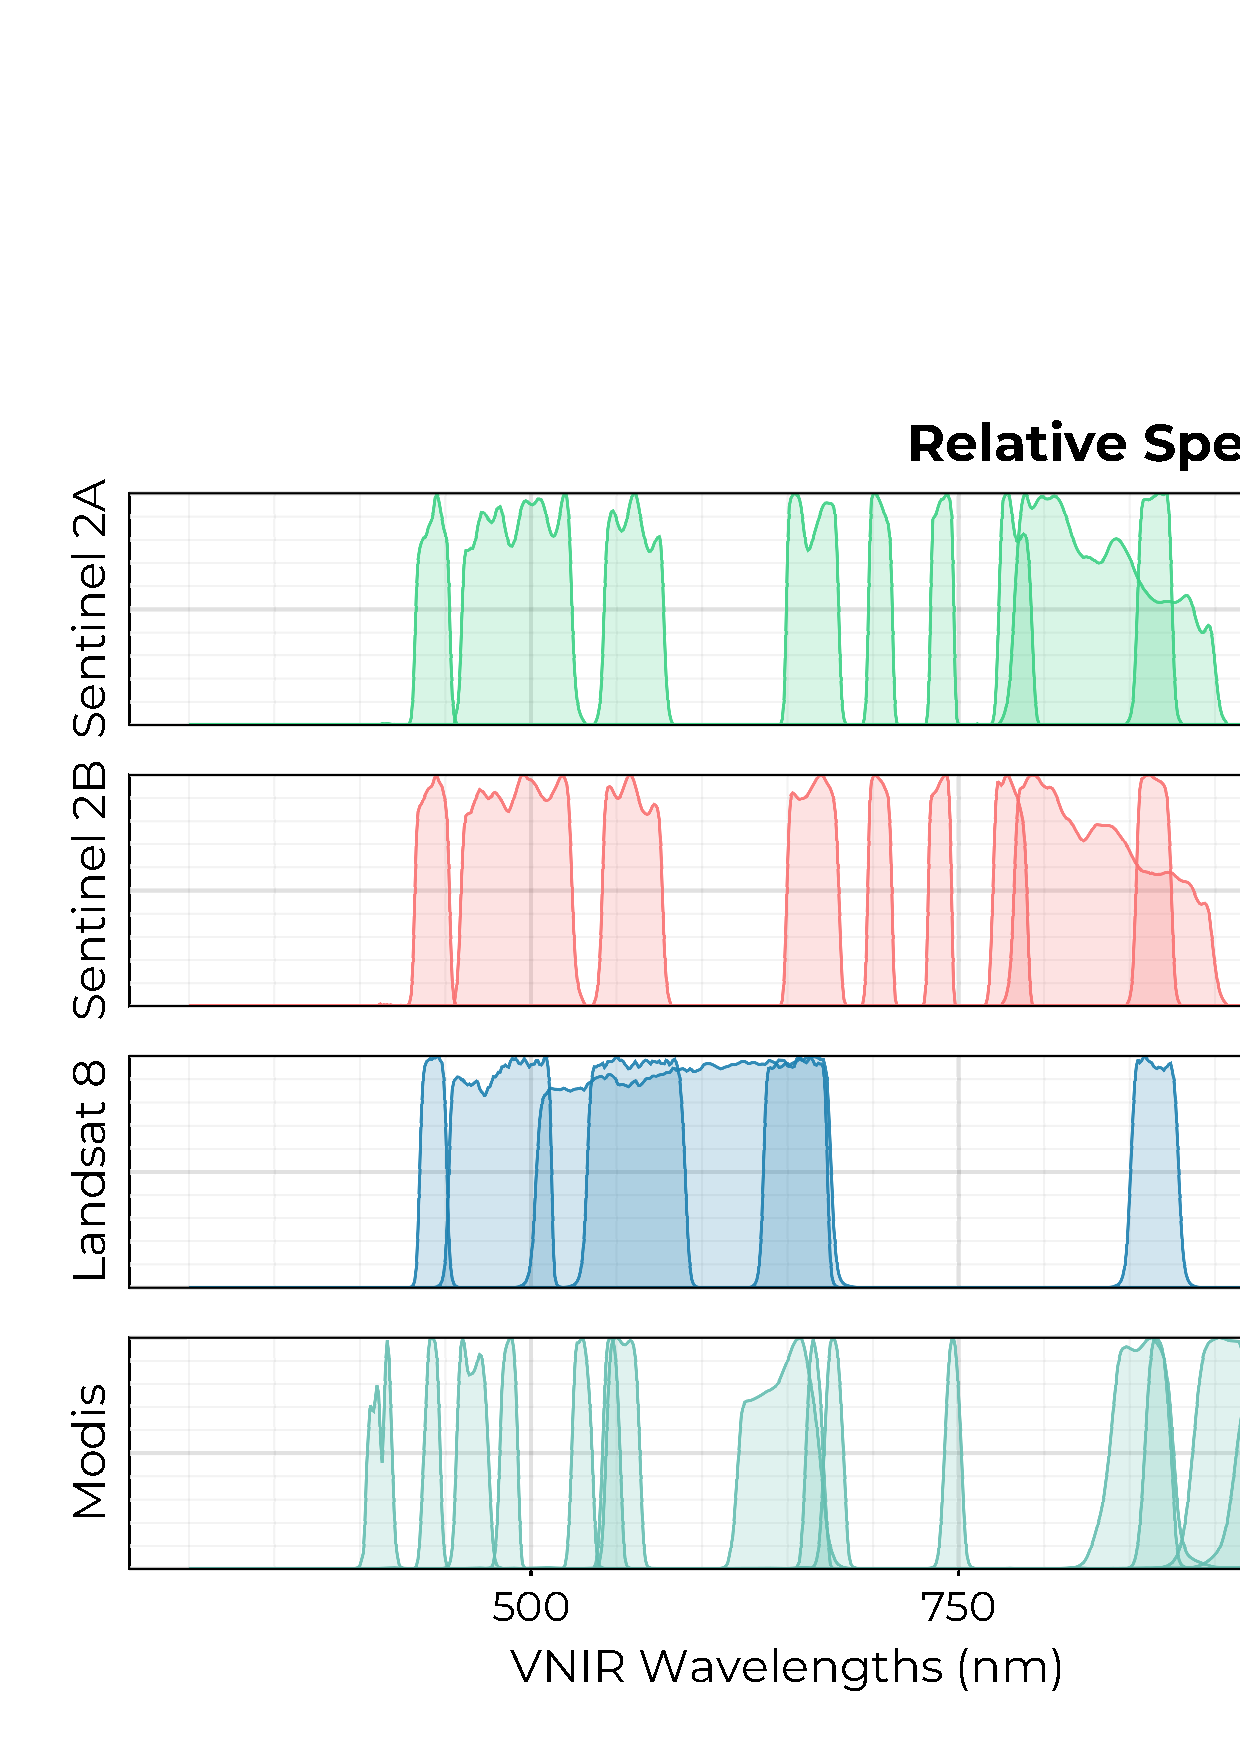
\includegraphics[width=0.85\columnwidth]{robot-team/passbands.pdf}
  \caption{A comparison of the relative spectral response for the passbands of popular multi-spectral imaging remote sensing platforms.}
  \label{fig:passbands}
\end{figure}

Many currently used spectral indices like the normalized difference vegetation
index (NDVI) take advantage of spectral features by comparing ratios of
pigment sensitive passbands to the stable signals in the infrared to infer the
abundance of chlorophyll, and consequently, the health of plants
\cite{ndvi-chlorophyll}.  However, despite the many successful
applications of multi-spectral imaging, there are a few key limitations which
impact their use for the assessment of water quality.

\begin{enumerate}
  \item Multi-spectral imagers have limited use for the assessment of many
    constituents affecting water quality whose spectral features overlap in the
    broad wavelength bands of systems like those shown in Figure~\ref{fig:passbands}.
  \item Satellite-based instruments measure top of atmosphere reflectance and
    must be carefully corrected to obtain values at the surface by accounting for
    absorption and scattering by atmospheric gases and particulates.
  \item Validating models which map remotely sensed reflectance to parameters of
    interest requires the collection of in situ reference data. This relies on
    serendipetous satellite passes over sensing sites often requiring decades of
    observations to collect sufficient quantities needed for model training and
    validation \cite{aurin2018remote, ross2019aquasat}.
\end{enumerate}

Hyperspectral imagers are designed to measure spectral radiance for many
hundreds of wavelengths at each image pixel. Their improved spectral resolution
makes it possible to detect fine spectral features. Developments in
hyperspectral imaging technology have led to dramatic reductions in both their
size and weight so that it is now possible to incorporate the
technology as the payload of highly mobile unmanned aerial vehicles (UAV) such as
drones. By collecting hyperspectral images (HSI) close to the ground, we limit
the need for complicated atmospheric corrections while enabling centimeter-scale
spatial resolutions. However, the massive size of HSI poses a significant
computational challenges for their adoption in real-time
applications.

The typical timescale from starting work on a new remote sensing data
product to its operational readiness is at least a couple of years, but, more
typically, a decade or more. Our goal is to reduce this timescale to be near
real time by utilizing an autonomous robotic team that can both collect the
training data, and then in real time process and stream the remote sensing data
products. The fully autonomous team includes an uncrewed surface vessel (USV)
that carries a suite of sensors to measure in situ water composition,
and an autonomous UAV equipped with a hyperspectral imager, downwelling
irradiance spectrometer, thermal imagers, and embedded compute for onboard machine
learning capabilities. Figure \ref{fig:drone-team} shows photographs of the robot team
during a deployment in North Texas.

\begin{figure}[!hbt]
  \centering
  \includegraphics[width=0.9\columnwidth]{robot-team/robot-team-photos.png}
  \caption{The autonomous robotic team. (\textbf{left}) The drone hovering a few
  feet above the ground during take-off. (\textbf{center}) the USV deployed in
  the water. (\textbf{right}) The drone as seen from below.}
  \label{fig:drone-team}
\end{figure}

The autonomous boat used is a
\href{https://www.maritimerobotics.com/otter}{Maritime Robotics Otter }. With a
footprint of only 200 × 108 × 81.5 cm, a weight of 55 kg, and dual electrical
fixed thrusters, it is an easily deployable asset that can be transported in a
van or even within normal airliners to a survey site. At a cruise speed of two
knots, it has a duration of approximately 20 hours per battery charge. It can use
WiFi, cellular, and an optional AIS receiver for communication to the control
station. Our drone is a \href{https://freeflysystems.com/alta-x}{Freefly Alta-X}
professional quad-copter. It was specifically designed to carry cameras, with a
payload capacity of up to 35 lb, a long range data link, and autonomy provided
by the Open PX4 flight stack. The open source QGroundControl software is used to
control the autonomous operations.

Both the UAV and USV carry high-accuracy GPS and inertial
measurement units (IMU) so that every data point can be georeferenced and time
stamped. Each robot can also join the same wireless network which connects the
robots and a ground control stations. For the deployments described in
Chatpers~\ref{ch:robot-team-supervised}, \ref{ch:robot-team-gtm}, and
\ref{ch:robot-team-gsm}, long-range
\href{https://www.ui.com}{Ubiquiti 5 GHz LiteBeam airMAX WiFi} was used for
data transfer and control. The network
also includes a local \href{https://www.synology.com}{Synology network-attached
  storage (NAS)} device which syncs collected data to another NAS in our home laboratory at the
UT Dallas for redundancy.

The robotic boat payload includes a
\href{https://www.biosonicsinc.com/products/mx-aquatic-habitat-echosounder/}{BioSonics
  MX Aquatic Habitat Echosounder sonar} for rapid assessment and mapping of
aquatic vegetation, substrate and bathymetry. Three
\href{https://www.waterprobes.com/multiprobes-and-sondes-for-monitori}{Eureka
  Manta-40 multi-probes}, a
\href{https://www.sequoiasci.com/product/lisst-abs/}{Sequoia Scientific
  LISST-ABS acoustic backscatter sediment sensor}, and an
\href{https://www.airmar.com/weather-description.html?id=153}{Airmar Technology
  Corporation 220 WX ultra-sonic weather monitoring sensor}.

The first Manta-40 multi-probe includes sensors for temperature and turbidity
and
\href{https://www.turnerdesigns.com/cyclops-7f-submersible-fluorometer}{Turner
  Designs Cyclops-7 submersible Titanium body fluorometers} for chlorophyll a,
chlorophyll a with red excitation, blue-green Algae for fresh water
(phycocyanin), blue-green Algae for salt water (phycoerythrin), and CDOM.
The second Manta-40 multi-probe includes sensors for temperature, conductivity
(with specific conductance, salinity, and total dissolved solids, TDS), pH (with
separate ref-erence electrode), optical dissolved-oxygen, turbidity, and ion
selective electrodes by Analytical Sensors and Instruments
(\url{http://www.asi-sensors.com/}, accessed 05/01/2021) for ammonium
(\ce{NH4^+}), bromide (\ce{Br^-}), calcium (\ce{Ca^2+}), chloride (\ce{Cl^-}),
nitrate (\ce{NO3^-}), and sodium (\ce{Na^+}). The third Manta-40 multi-probe
includes sensors for temperature, turbidity, a total dissolved gas sensor, and
additional fluorometers for measuring optical brighteners, crude oil, refined
fuels, and tryptophan.

\begin{figure}[!hbt]
  \centering
  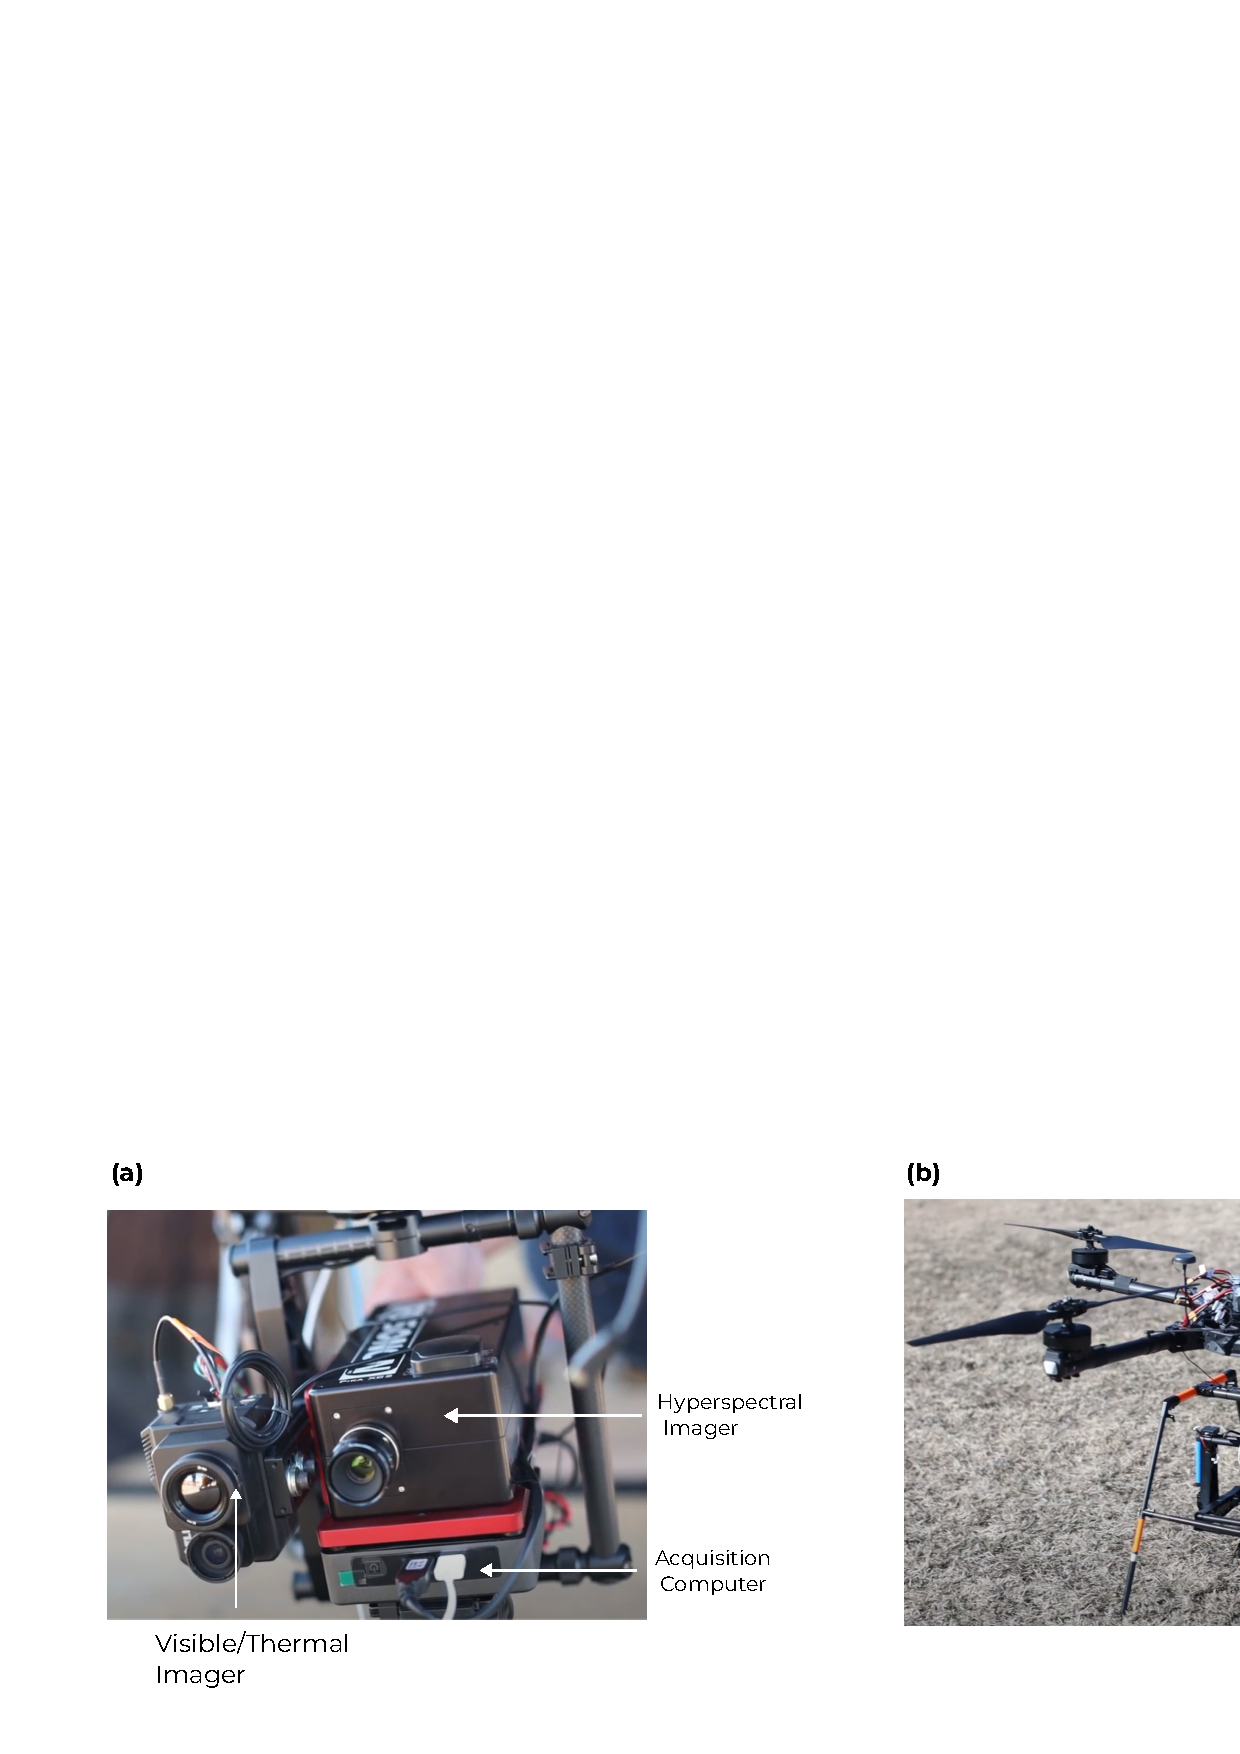
\includegraphics[width=0.9\columnwidth]{robot-team/annotated-drone.pdf}
  \caption{An annotated view of the autonomous drone showcasing the hyperspectral imager and onboard compute.}
  \label{fig:uav-closeup}
\end{figure}

Custom landing gear gear made from light-weight
carbon fiber was manufactured for the UAV to maximize the potential carry
capacity. The installed hyperspectral imager is a
\href{https://resonon.com/Pika-XC2}{Resonon Visible+Near-Infrared (VNIR) Pika
  XC2}, and thermal images are captured with
a \href{https://www.flir.com/products/duo-pro-r/}{FLIR Duo Pro R} installed
in a parallel configuration as indicated in Figure~\ref{fig:uav-closeup}. On top
of the UAV, a sky facing Ocean Optics UV-Vis-NIR spectrometer with an included
cosine corrector measures the incident downwelling irradiance to enable the
conversion of radiance hyperspectral data cubes to reflectance.

During a single 30 minute deployment, the robot team is able to autonomously
collect over a terabyte of HSIs together with over 10,000 in situ measurements
from the suite of sensors on the USV. Coordinating UAV flights to overlap USV
data collection makes it easy to identify reflectance spectra collocated with
USV measurements. This in turn makes it possible quickly train machine learning
models mapping HSI reflectance spectra to water quality parameters of interest.
Once trained, the models may be deployed directly onto the UAV computer to allow
streaming of concentration maps to the ground station during subsequent flights.
The machine learning models developed for the robot team are described in
Chapter~\ref{ch:robot-team-supervised}. Additionally, unsupervised techniques
for assessing the presence of unanticipated contaminants are developed in
Chapters~\ref{ch:robot-team-gtm} and
\ref{ch:robot-team-gsm}.

In the final sections of this chapter, we present the methods implemented to
rapidly georectify captured HSI and convert their radiance measurements to
reflectance using secondary spectra from the downwelling irradiance
spectrometer. This process quickly assigns latitude and longitude coordinates to
each HSI pixel making it possible to generate maps of the reflectance
distribution across an entire body of water. The coordiantes of georectified HSI
are also used to collocate reflectance spectra with in situ USV measurements.



\section{Rapid Processing and Georectification of Hyperspectral Data Cubes}

For an HSI platform to operate in (near) real-time, three key tasks are critical:
\begin{enumerate}
\item \textbf{FileIO}: Raw HSI need to be quickly read by the on-board processing computer.
\item \textbf{Georectification}: HSI must be georeferenced so that each image
  pixel can assigned a location on the ground.
\item \textbf{Radiometric Conversion}: HSI data cubes need to converted to the
  desired radiometric quantity, i.e. the reflectance.
\end{enumerate}

The first item is readily accomplished by means of light-weight, high-volume
solid state drives incorporated into the UAV computer. To address the second, we
need both sufficient compute capabilities and optimized processing software. The
final item relies on both the georectified data cube and the secondary
irradiance spectrum captured by the upward facing downwelling irradiance
spectrometer. To enable this workflow, the UAV utilizes a pair of light-weight
processing computers (Intel NUCs) each have 12 cores and 64 gigabytes of
installed RAM.  One is attached directly to the imager and
manages data acquisition by the camera and saving of raw HSI files. The second
NUC is mounted above the payload and serves as the onboard data processing unit. These
computers can be seen in panels (a) and (b) of Figure~\ref{fig:uav-closeup}.

%The upward facing spectrometer captures the \textit{downwelling} irradiance
%spectrum, $E_d(\lambda)$ which is necessary to enable conversion from radiance units to the

The georectification procedure implements for HSI from the UAV is based on the
methods described in \cite{muller2002program, baumker2001new, mostafa2000multi}
for pushbroom-mode hyperspectral imagers while the reflectance conversion
assumes Lambertian scattering as described previously in Section~\ref{sec:imaging}.
The processing steps are as follows:

\begin{enumerate}
\item Raw imagery (radiance spectra) are continuously captured by the hyperspectral imager and stored in binary ENVI format.
\item The processing computer read an ENVI file into a multi-dimensional array
  once it finishes writing.
\item Associated flight data (GPS and IMU) are read.
\item Flight data are interpolated to match the sample times for each HSI scan-line.
\item Each scan-line is georeferenced to obtain coordinates (lat,lon) for each pixel.
\item The georeferenced HSI is then resampled to a regular grid spatial grid.
\item The downwelling irradiance spectrum associated with the HSI is read.
\item The downwelling spectrum is interpolated to match the wavelength bins of the HSI
\item The HSI is converted o reflectance.
\item Spectral indices (NDVI, etc...) are computed.
\item The final data cube is saved to an HDF5 file.
\end{enumerate}
A visual representation of the pipeline is shown in
Figure~\ref{fig:hsi-pipeline} below.
\begin{figure}[H]
  \centering
  \includegraphics[width=\columnwidth]{robot-team-supervised/materials-and-methods/pipeline-figure-2.pdf}
  \caption{Hyperspectral image processing: Hyperspectral data cubes are
    collected one scan-line at a time (left). By utilizing downwelling
    irradiance spectra, we convert each pixel from spectral radiance to
    reflectance. By using orientation and position data from the on-board GPS
    and INS, we georeference each pixel to assign it a latitude and longitude on
    the ground. The final data product is the georectified hyperspectral
    reflectance data cube (right) visualized as a pseudo-color image with
    reflectance  as a function of wavelength along the
    z-axis.\label{fig:hsi-pipeline}}
\end{figure}


% \begin{figure}[h]
%   \centering
%   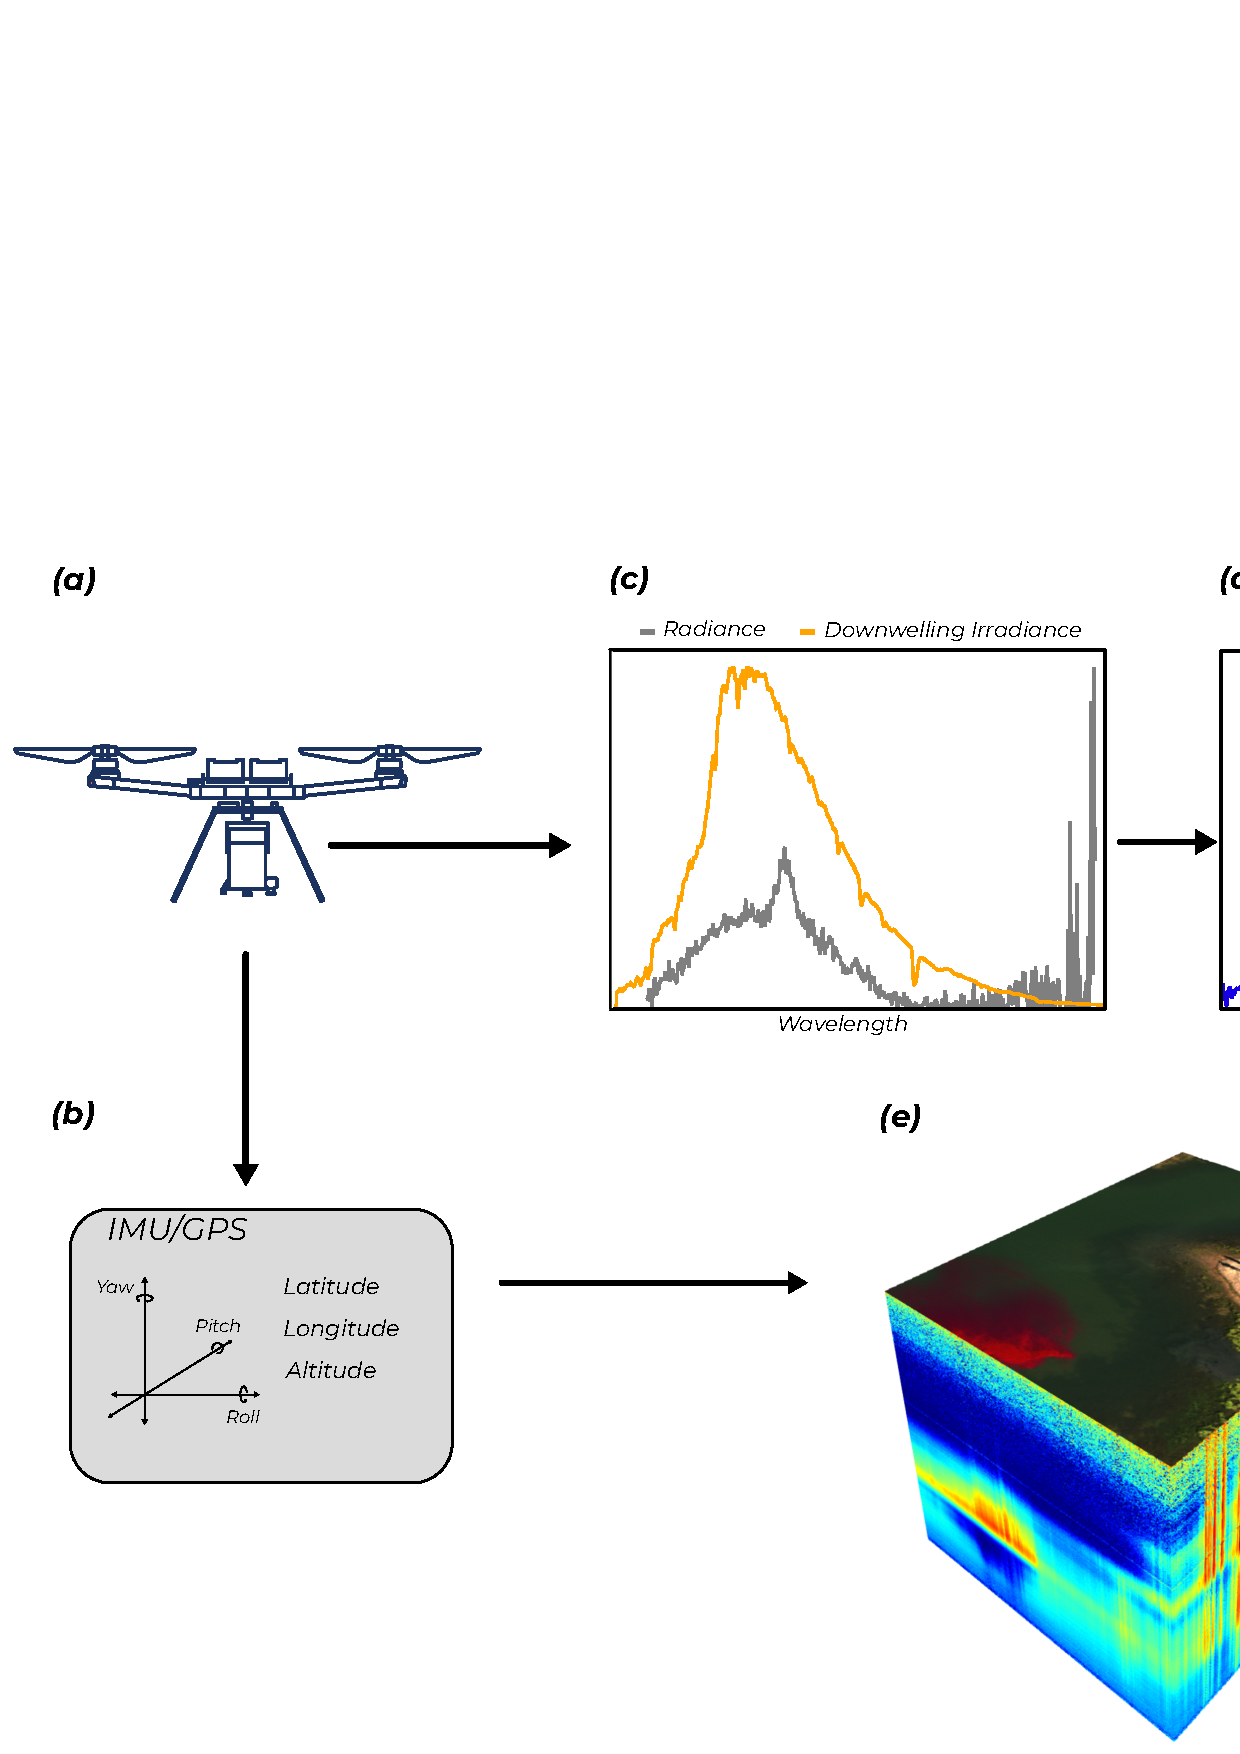
\includegraphics[width=0.85\columnwidth]{robot-team/georectification/pipeline-figure.pdf}
%   \caption{Visual representation of the HSI processing pipeline. HSI images from
%   the UAV (a) are georectified using position and orientation data from the
%   embedded GPS/IMU unit (b). Pixel radiance spectra are combined with
%   downwelling irradiance (c) to yield a reflectance spectrum for each pixel (d).
%   The result is a georectified reflectance data cube (e).}
%   \label{fig:hsi-pipeline}
% \end{figure}


\subsection{Georeferencing and Resampling}

The hyperspectral imager used on the UAV is different from a typical camera;
instead of capturing an image by sampling light across array of sensors, the
hyperspectral imager uses a pushbroom configuration. In this setup, a single
scan-line of pixels is captured by the sensor for each wavelength and an image
is formed as the drone flies along its route. This poses an interesting
challenge for georeferencing as each individual scanline must be transformed
independently. As the drone's path winds and turns, each scanline
is stretched and rotated based on the relative orientation of
the drone to the ground at the time of capture. This sampling geometry as well
as the relevant orientation angles are illustrated in Figure
\ref{fig:georectification}.

\begin{figure}[h]
  \centering
  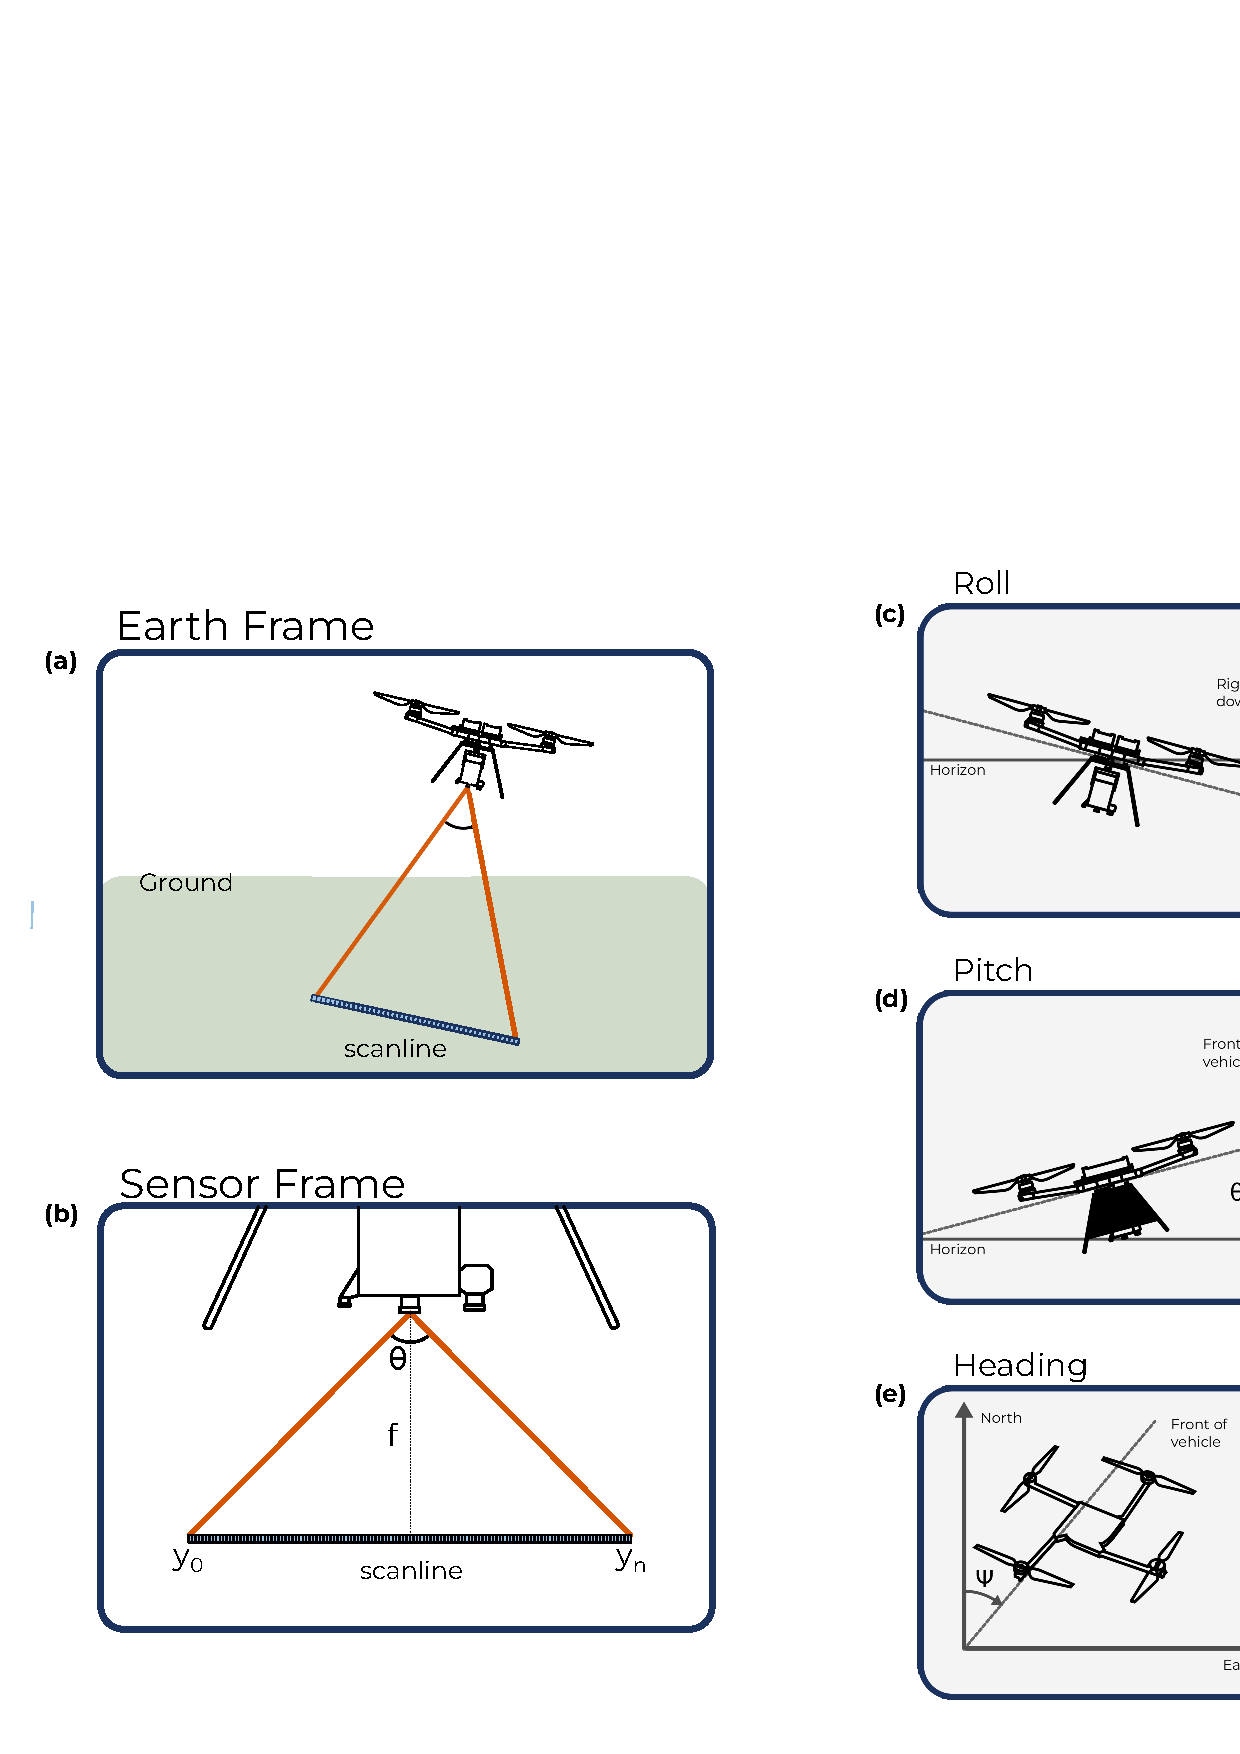
\includegraphics[width=0.95\columnwidth]{robot-team/georectification.pdf}
  \caption{Visual representation of sampling geometry for the UAV. (\textbf{a})
    the scan-line as seen from the Earth frame. (\text{b}) the HSI scan-line as
    represented in the frame of the sensor. (\textbf{d, d, e}) The angles
    describing the orientation of the drone in flight.}
  \label{fig:georectification}
\end{figure}

The GPS and IMU on the hyperspectral imager continuously capture the location $(\lambda,
\Phi, z)^T$  (longitude, latitude, altitude) of our drone as well it's
orientation defined by the angles $\phi$, $\theta$, and  $\psi$ (roll, pitch,
and heading). To georeference each pixel, we therefore must transform its
position from the frame of the sensor (measured in pixels relative to the
imager's sensor) first to the frame of the IMU used to measure the orientation,
then to the navigation frame (East, North, up), and finally to the ground frame. Let us
define the \textit{sensor} frame so that the scan-line falls upon the y axis. As
each scanline must be transformed independently, we can assign it an
x-coordinate of $0$ pixels. Lastly, if the viewing angle of the HSI is
$\theta_{\text{view}}$, then the coordinates of the i-th pixel,
$\mathbf{r}_i^{\text{sensor}}$, in the sensor frame are defined as in panel (b)
of Figure \ref{fig:georectification} to be
\begin{equation}
  \mathbf{r}_i^{\text{sensor}} = \left[ 0, y_i, f \right]^T
\end{equation}
where $y_i\in \left\{-\frac{(N-1)}{2},...,\frac{N-1}{2}\right\}$ and
$f=\frac{(N-1)/2}{\tan(\theta_{\text{view}}/2)}$ for $N$-total pixels per
scan-line. To align the sensor frame with the axes of
the IMU, we apply a sequence of rotation matrices defined using the measured
orientation angles (panels (c), (d), and (e) of Figure
\ref{fig:georectification}), denoted by
\begin{equation}
  \begin{aligned}
    &\mathbf{R}_{\text{sensor}}^{\text{IMU}}(\phi,\theta,\psi) = \\
    &\begin{bmatrix}
    \cos(\psi)\cos(\theta) & \cos(\psi)\sin(\theta)\sin(\phi)-\sin(\psi)\cos(\phi) & \cos(\psi)\sin(\theta)\cos(\phi)+\sin(\psi)\sin(\phi) \\
    \sin(\psi)\cos(\theta) & \sin(\psi)\sin(\theta)\sin(\phi)+\cos(\psi)\cos(\phi) & \sin(\psi)\sin(\theta)\cos(\phi)-\cos(\psi)\sin(\phi) \\
    -\sin(\theta) & \cos(\theta)\sin(\phi) & \cos(\theta)\cos(\phi)
     \end{bmatrix}.
  \end{aligned}
\end{equation}

Next, an orthogonal transformation is applied to transform from the IMU frame to
the navigation frame of the drone. This is important as the axes of the IMU and
the drone itself are not necessarily identical depending on how the IMU is
oriented on the HSI. For the UAV, this amounts to
\begin{equation}
  \mathbf{T}_{\text{IMU}}^{\text{DRONE}} = \begin{bmatrix}
    0 & 1 & 0 \\
    1 & 0 & 0 \\
    0 & 0 & -1
    \end{bmatrix}.
\end{equation}
At this stage, the pixel coordinates have been rotated into the frame of the
drone and must be rescaled from pixel units to meters. This is accomplished by
observing that panels (a) and (b) of Figure~\ref{fig:georectification} form
similar triangles with an shown in Figure~\ref{fig:s-geom}.

\begin{figure}[h]
  \centering
  \includegraphics[width=0.6\columnwidth]{robot-team/scale-factor-geometry.pdf}
  \caption{At a height $\Delta z$, the position of an HSI pixel in the Earth
    frame depends on the roll $\theta$ and pitch $\phi$.}
  \label{fig:s-geom}
\end{figure}

For a height $\Delta z = z-z_{\text{ground}}$ above the ground, the distance $L$ from
the camera to an HSI pixel on the ground is
\begin{align*}
  L &= \sqrt{\Delta z^2 + \ell^2} \\
    &= \sqrt{\Delta z^2 + \Delta z^2\tan^2\theta + \Delta z^2\tan^2(-\phi)} \\
    &= \Delta z \sqrt{1 + \tan^2\theta + \tan^2\phi}
\end{align*}
leading to a scale factor
\begin{equation}
  s = \frac{L}{f} = \frac{\Delta z}{f}\sqrt{1 + \tan^2\theta + \tan^2\phi}.
\end{equation}

Finally, the coordinates of each pixel are translated using the position of the
drone in the chosen coordinate system. As the geometric transformations are
scaled to units of meters (by $s$), a coordinate transformation $f$ is applied to
obtain the position of the drone with respect to a local coordinate system such
as the Universal Transverse Mercator (UTM). Written all together, this becomes
\begin{equation}\label{eq:georec-eqn}
  \mathbf{r}_{i}^{\text{UTM}} =
  f_{\text{geo}}^{\text{UTM}}\begin{bmatrix}
    \lambda \\
    \Phi \\
    z_{\text{drone}}
  \end{bmatrix}_{\text{GPS}}^{\text{geo}} + s\mathbf{T}_{\text{IMU}}^{\text{DRONE}}\mathbf{R}_{\text{sensor}}^{\text{IMU}}(\theta, \phi, \psi)\begin{bmatrix}
    0 \\
    y_i \\
    f
  \end{bmatrix}^{\text{sensor}}
\end{equation}

The transformation from Equation~\ref{eq:georec-eqn} is applied \textit{in parallel}
to each scan-line to obtain the ground coordinates $\mathbf{r}_i=(x_i,
y_i,z_i)^T$ of each pixel. Finally, the resulting HSI is resampled to a
rectangular grid at a specified resolution by rounding each pixel's
coordinates to the desired accuracy and averaging all spectra that fall within the
same grid cell. Adjusting the final resolution of the georectified data cube
allows for optimization of compute time against spatial scale for real time
applications.

\subsection{Reflectance Conversion}

Once an HSI is georeferenced and resampled to the desired scale,
the downwelling irradiance spectrum measured during HSI acquisition is used to
convert the raw data from radiance to reflectance. This effectively normalizes
the HSI by \textit{dividing out} the incident light distribution making it possible
to compare spectra captured under variable lighting conditions. First,
the downwelling irraidance spectrum is loaded and interpolated to match the
wavelengths of the spectral bins of the hyperspectral imager. The reflectance at
pixel $(i,j)$ and wavelength $\lambda_k$ is then obtained by
\begin{equation}
  \rho_{ijk} = \frac{\pi L_{ijk}}{E_k}
\end{equation}
where $L_{ijk}$ denotes the original radiance pixel at wavelength bin $k$ and
$E_k$ denotes the downwelling irradiance at wavelength $\lambda_k$.

\begin{figure}[h]
  \vspace{-2cm}
  \centering
  \includegraphics[width=0.55\columnwidth]{robot-team/georectification/demo-rectified-cube.png}
  \vspace{-1cm}
  \caption{Example of a georectified reflectance data cube. A pseudo color image is
    included at the top of the image showing what an observer would see from the
    perspective of the UAV. The log-10 reflectance is plotted at each wavelength
    bin along the z-axis. }
  \label{fig:sample-cube}
\end{figure}

Figure \ref{fig:sample-cube} illustrates an example of a georectified
reflectance data cube. The spectral signature corresponding to
a Rhodamine tracer dye released into the water is clearly visible in the front
left portion of the image.

\subsection{Timing Results}

This processing pipeline was implemented in the Julia programming language and
the associated code is accessible at \url{github.com/john-waczak/RobotTeam.jl}.
Using the package \texttt{BenchmarkTools.jl}, the time to load and georeference
HSI using the UAV processing computer for HSI with 371, 462, and 1000 scan-lines are
shown in Table~\ref{tab:georeference-times}.

\begin{table}[!hbt]
  \caption{Loading and georeferencing time as a function of number of scan-lines}
  \label{tab:georeference-times}
  \centering
  \begin{tabular}{cc}
    \hline
    \textbf{Number of scan lines}	& \textbf{Execution time (s)}\\
    \hline
    371		  &   0.161	\\
    462     &   0.197	\\
    1000    &   0.195  \\
    \hline
  \end{tabular}
\end{table}

The total processing time including resampling and conversion to reflectance as a
function of final resolution is shown in Figure~\ref{fig:regridding-timing} for
an HSI of initial size $1000\times 1600 \times 462$.

\begin{figure}[!hbt]
  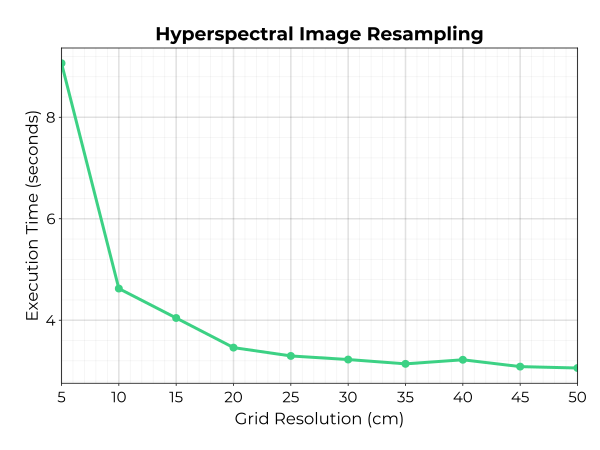
\includegraphics[width=0.85\columnwidth]{robot-team/georectification/regrid-timing.pdf}
  \caption{Timing results (in seconds) for resampling a 1000 scanline HSI as a function of output grid resolution.}
  \label{fig:regridding-timing}
\end{figure}

These timings indicate that processing an HSI to a final spatial resolution of
$20$ cm takes less than $4$ seconds which is comparable to the acquisition rate
of the hyperspectral imager. The key limitation of this implementation is the
assumption that the ground is flat. However, the studies in this dissertation
are focus specifically on imaging over the water where this approximation is
reasonable. For processing HSI collected over rough terrain, a digital elevation
map (DEM) can be used to augment the georectification process. Future iterations
of the drone can include small form-factor computers with integrated graphics
processing units (GPU) to accelerate these calculations. Here the problem of
georectification can be recast into a ray-tracing problem for each pixel
\cite{gpu-georect}.
